\documentclass[a4paper, 10pt]{article}

\usepackage[utf8]{inputenc}
\usepackage[spanish]{babel}
\usepackage{graphicx}
\usepackage{geometry}
\usepackage{listings}
\usepackage{amsmath}
\usepackage{amsfonts}
\usepackage{amssymb}
\usepackage{caratula}
\usepackage[section]{placeins}
\usepackage{titlesec}

\newcommand{\Z}{\mathbb{Z}}
\def\code#1{\texttt{#1}}
\newcommand\tab[1][0.5cm]{\hspace*{#1}}

\geometry{a4paper, margin=0.7in}

\begin{document}
    %Caratula
    \pagenumbering{gobble}
    \newpage

    \begin{center}
        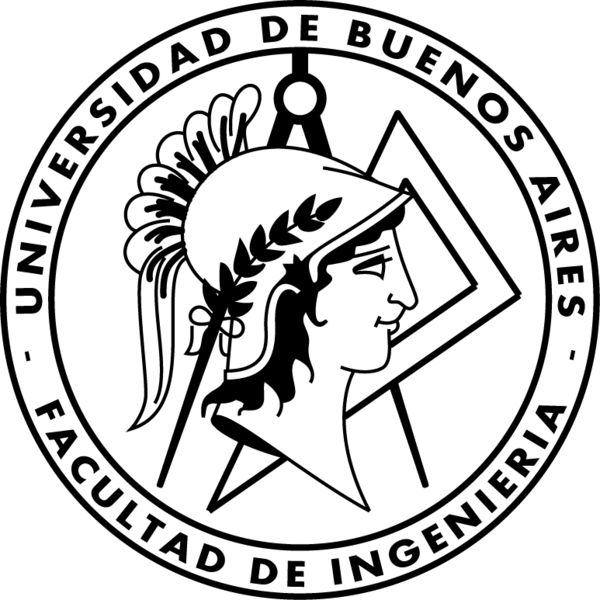
\includegraphics[width=7.5cm, height=7.5cm]{images/logo}
    \end{center}

    \materia{Organización de Datos}
    \submateria{Segundo Cuatrimestre 2017}
    \titulo{Trabajo Práctico 1}

    \integrante{Rodrigo De Rosa}{97799}{rodrigoderosa@outlook.com}
    \integrante{Marcos Schapira}{97934}{schapiramarcos@gmail.com}
    \integrante{Facundo Guerrero}{97981}{facundoiguerrero@gmail.com}
    \maketitle
    %Fin caratula
    %Table of contents
    \newpage
    \pagenumbering{roman}
    \tableofcontents
    %Fin table of contents
    %Informe
    \newpage
	\pagenumbering{arabic}
	\part{Análisis del tipo de las propiedades}
		En esta parte, se analizará como las distintas características de las propiedades son afectadas por el tipo de propiedad.
		Esto es, si son negocios, casas, PHs o departamentos.
		\section{Tipos de propiedades y sus superficies}
			La idea de esta sección es analizar en que lugares podemos encontrar a las propiedades con mayor y menor superficie
			en CABA y GBA. \\
			\tab Se debe mencionar que para realizar este análisis nos quedamos sólo con ciertos barrios en base a la cantidad de
			propiedades de cada tipo que contienen. Este recorte se realizó de la siguiente manera:
			\begin{center}
				\begin{tabular}{ |c|c|c| }
					\hline
					\multicolumn{2}{|c|}{Recorte de barrios}\\
					\hline
					\hline
					Tipo & Cantidad mínima \\
					\hline
					Casa & 35\\
					Locales & 15\\
					Departamentos & 180\\
					PHs & 40\\
					\hline
				\end{tabular}
			\end{center}
			\subsection{¿Dónde están las propiedades más grandes según su tipo?}
				\subsubsection{Casas}
					En el caso de las casas, al hacer un \emph{Top 5}, obtenemos el siguiente resultado:
					\begin{center}
						\begin{tabular}{ |c|c|c| }
							\hline
							\multicolumn{3}{|c|}{Superficie promedio de las casas por barrio}\\
							\hline
							\hline
							Puesto & Barrio & Superficie [$m^2$]\\
							\hline
							1 & Benavidez & 718 \\
							2 & Parque Leloir & 530 \\
							3 & Maschwitz & 499 \\
							4 & Acassuso & 481 \\
							5 & Belén de Escobar & 455\\
							\hline
						\end{tabular}
					\end{center}
					\tab Se puede ver que las casas en estos cinco barrios son considerablemente grandes y que el primero, Benavidez,
					tiene un promedio mucho mayor que el segundo ($26\%$ más grande) mientras que entre los siguientes cuatro barrios
					la diferencia es menor. A continuación, veremos un gráfico de barras de estos primeros 5 barrios.
					\begin{center}
   		    				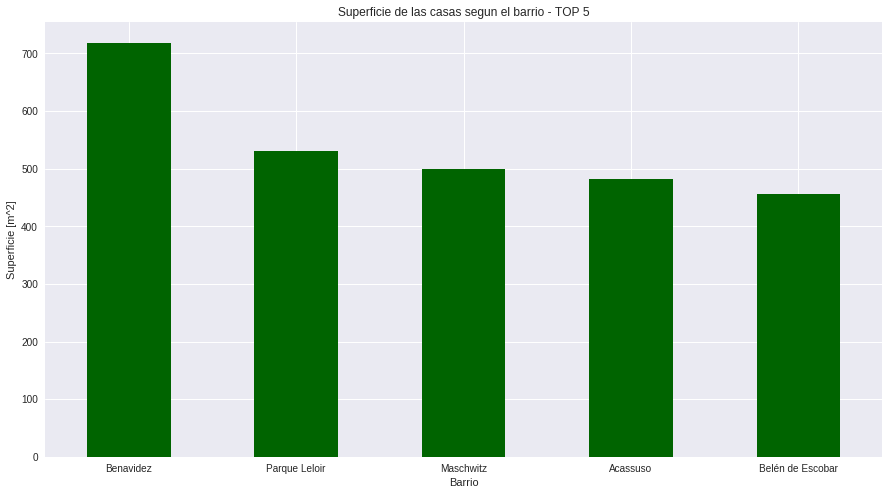
\includegraphics[width=\textwidth]{images/houseSurfaceTopBar}
				  	\end{center}
				  	\tab En este gráfico se ve lo mencionado previamente, una considerable diferencia entre el primero y el segundo
				  	y luego un descenso más estable. \\
				  	\tab Finalmente, veremos cuál es la ubicación geográfica de estas casas.
				  	\begin{center}
   		    				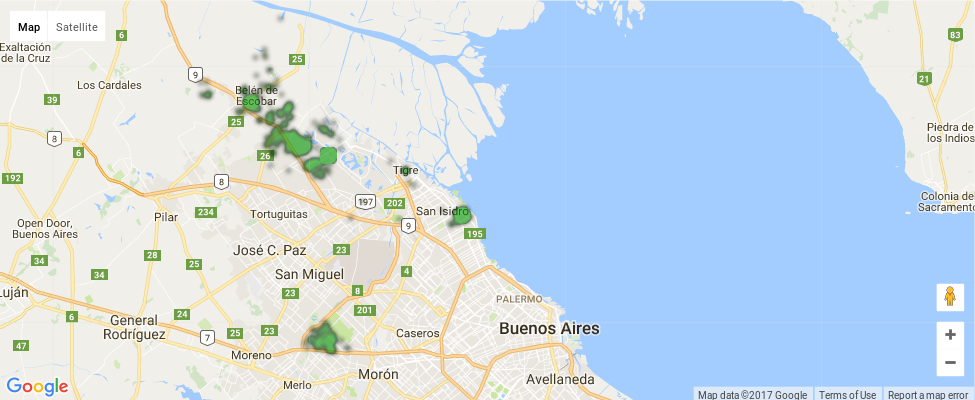
\includegraphics[width=\textwidth]{images/houseSurfaceTopMap}
				  	\end{center}
				  	\tab Se puede ver que, como era de esperar, son todos barrios alejados de la Capital Federal, principalmente en
				  	Zona Norte. \\
				  	\tab Podría decirse, entonces, que las casas más grandes se encuentran en la provincia de Buenos Aires. De todos
				  	modos, se espera encontrar barrios como Belgrano en los primeros puestos (en Belgrano R hay casas muy grandes) y,
				  	de hecho, es el décimo puesto.
				\subsubsection{PHs}
					Para los PHs, el \emph{Top 5} arroja los siguientes resultados:
					\begin{center}
						\begin{tabular}{ |c|c|c| }
							\hline
							\multicolumn{3}{|c|}{Superficie promedio de los PHs por barrio}\\
							\hline
							\hline
							Puesto & Barrio & Superficie [$m^2$]\\
							\hline
							1 & Caseros & 165\\
							2 & San Telmo & 160.4\\
							3 & Barracas & 159.9\\
							4 & Almagro & 142.7 \\
							5 & Ciudadela & 142.6\\
							\hline
						\end{tabular}
					\end{center}
					\tab En este caso vemos que la diferencia entre los primeros cinco barrios es muy pequeña, de hecho, entre el
					segundo y tercero y entre el cuarto y el quinto, la diferencia es menor de un metro cuadrado. Si vemos esto en
					un gráfico de barras:
					\begin{center}
   		    				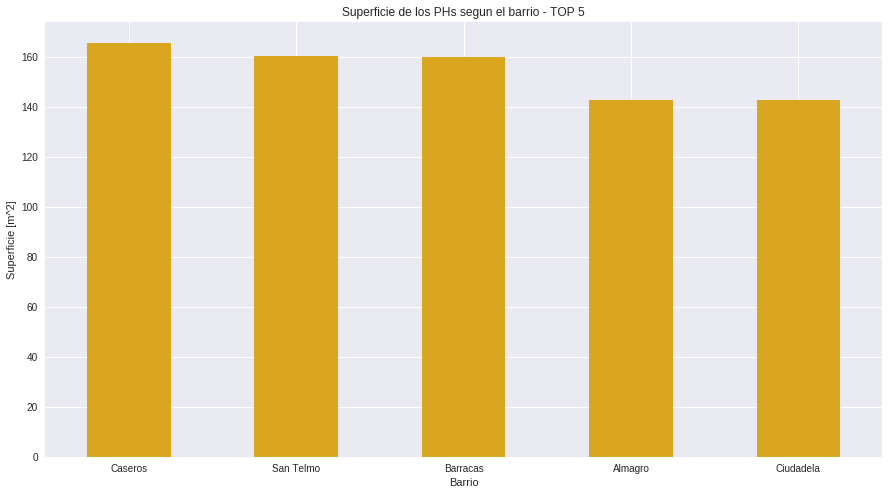
\includegraphics[width=\textwidth]{images/phSurfaceTopBar}
				  	\end{center}
				  	\tab Podemos ver la pequeña diferencia de superficie entre los primeros cinco barrios. Cabe destacar que la
				  	máxima superficie en este caso es el $23\%$ de la máxima superficie de las casas. \\
				  	\tab En cuanto a la ubicación geográfica de estos PHs, tenemos lo siguiente:
				  	\begin{center}
   		    				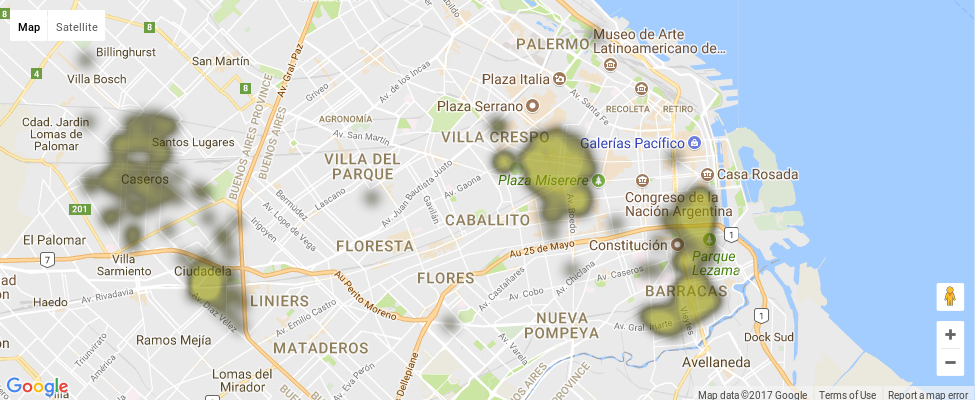
\includegraphics[width=\textwidth]{images/phSurfaceTopMap}
				  	\end{center}
				  	\tab Vemos que estos PHs se encuentran en Capital Federal y en dos barrios de la Provincia muy cercanos a CABA.
				  	Esto puede significar dos cosas; que simplemente los PHs más grandes están en la zona sur de CABA y algunos
				  	sectores de provincia o que es más común encontrar PHs en dichos lugares y no así en otros sectores de la ciudad,
				  	más alejados como con las casas, por lo que los primeros son los principales.
				\subsubsection{Departamentos}
					Para los primeros, el \emph{Top 5} es:
					\begin{center}
						\begin{tabular}{ |c|c|c| }
							\hline
							\multicolumn{3}{|c|}{Superficie promedio de los departamentos por barrio}\\
							\hline
							\hline
							Puesto & Barrio & Superficie [$m^2$]\\
							\hline
							1 & Palermo Chico & 177 \\
							2 & Puerto Madero & 150 \\
							3 & Retiro & 132 \\
							4 & Recoleta & 130\\
							5 & Barrio El Golf & 116\\
							\hline
						\end{tabular}
					\end{center}
					\tab Cabe destacar que en este caso no se unificaron los sectores de Palermo porque se consideró importante
					mostrar al barrio con los departamentos de mayor superficie promedio. \\
					\tab Al ver la tabla, encontramos cuatro barrios conocidos no solo como 'caros' en la Capital Federal sino
					también como el lugar de edificios grandes y lujosos, como es el caso de Puerto Madero y Retiro, por lo que
					no parece extraño encontrarlos en el \emph{Top 5}. El quinto puesto lo tiene un barrio cerrado de Tigre, donde
					también es de esperar que los departamentos sean grandes y lujosos. \\
					\tab El gráfico de barras en este caso nos muestra un descenso más abrupto que en el caso de los PHs y las casas.
					\begin{center}
   		    				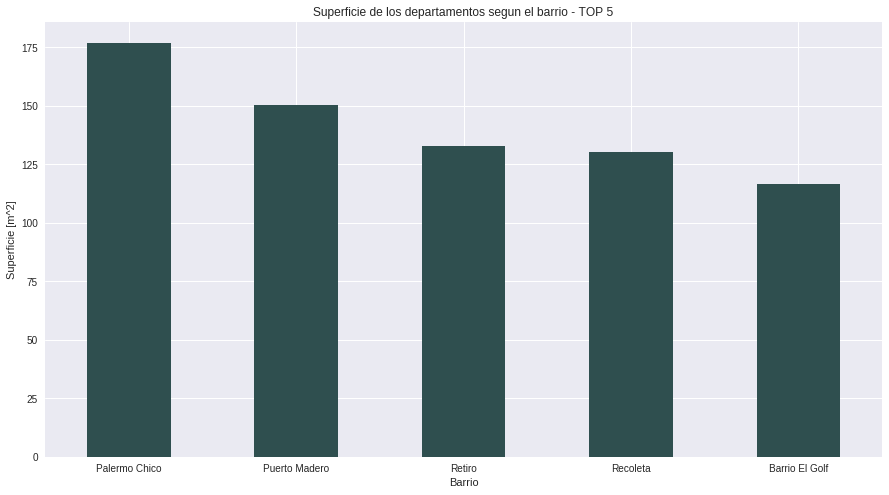
\includegraphics[width=\textwidth]{images/apartmentSurfaceTopBar}
				  	\end{center}
				  	\tab Vemos también que las superficies, en el caso de los máximos, son muy similares a las de los PHs (y por ende
				  	mucho menores que las de las casas). \\
				  	\tab Para la visualización de la ubicación geográfica no tuvimos en cuenta a el Barrio El Golf, pues por estar
				  	tan alejado de Capital Federal, no permite crear un gráfico entendible y útil.
				  	\begin{center}
   		    				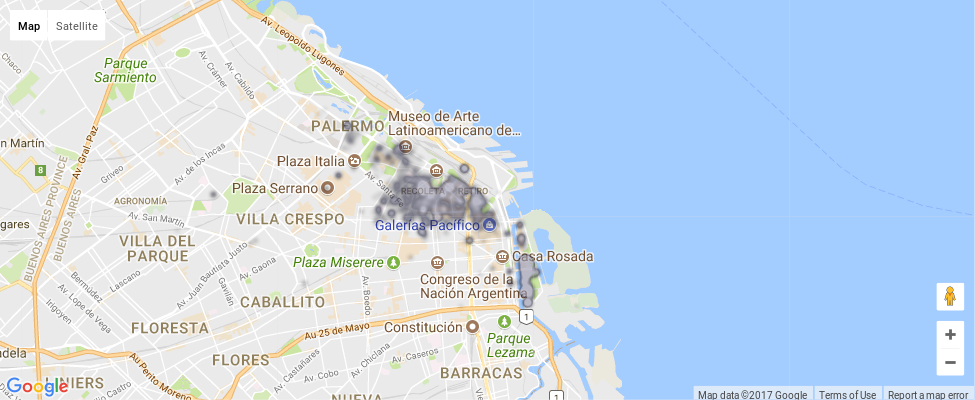
\includegraphics[width=\textwidth]{images/apartmentSurfaceTopMap}
				  	\end{center}
				  	\tab Vemos entonces que los departamentos con mayor superficie promedio se encuentran en aquellos barrios donde
				  	el precio por $m^2$ promedio también es el máximo. Esto se debe, como se dijo antes, a el 'alto nivel' de la
				  	zona, donde los edificios son lujosos y con muchos servicios y los departamentos suelen ser pisos o semi-pisos.
				\subsubsection{Locales}
					Finalmente, el \emph{Top 5} de los locales es el siguiente:
					\begin{center}
						\begin{tabular}{ |c|c|c| }
							\hline
							\multicolumn{3}{|c|}{Superficie promedio de los locales por barrio}\\
							\hline
							\hline
							Puesto & Barrio & Superficie [$m^2$]\\
							\hline
							1 & Martínez & 259\\
							2 & Caballito & 232\\
							3 & Balvanera & 231\\
							4 & San Telmo & 219\\
							5 & Microcentro & 217\\
							\hline
						\end{tabular}
					\end{center}
					\tab Aquí nos encontramos con un primer puesto no esperado. Pues si bien Martínez tiene una zona comercial, no
					se esperaba que fuera el que tiene los locales más grandes en promedio. Por otro lado, la aparición de los
					barrios céntricos no nos sorprende, dado que allí hay un polo comercial muy importante y con locales de gran
					superficie. De todas formas, más adelante analizaremos los barrios en los que hay mayor cantidad de locales (o
					de cada tipo de propiedad, mejor dicho). \\
					\tab Si vemos el gráfico de barras:
					\begin{center}
   		    				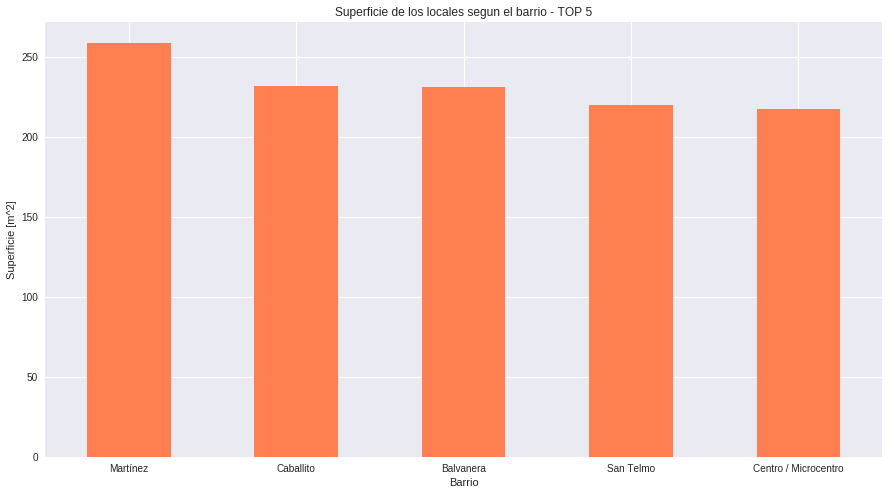
\includegraphics[width=\textwidth]{images/storeSurfaceTopBar}
				  	\end{center}
				  	\tab Vemos que la diferencia entre los primeros cinco barrios es pequeña y que, en promedio, los locales son
				  	más grandes que los departamentos y PHs, al analizar a los cinco más grandes de cada uno. \\
				  	\tab En cuanto a la ubicación geográfica:
				  	\begin{center}
   		    				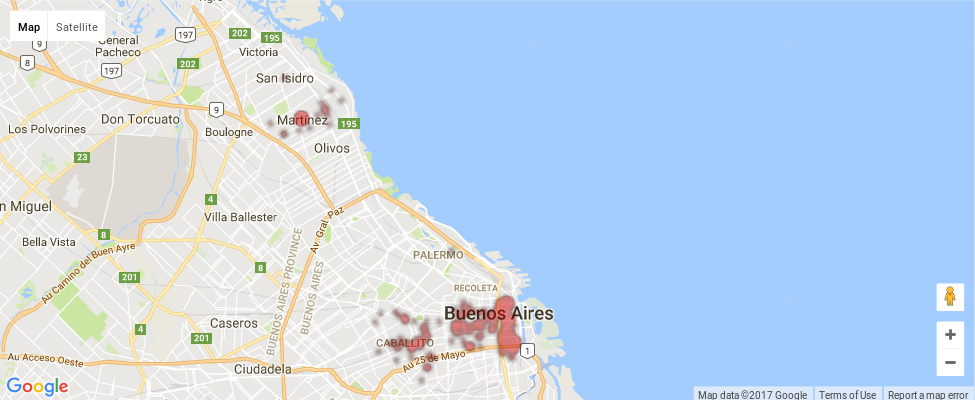
\includegraphics[width=\textwidth]{images/storeSurfaceTopMap}
				  	\end{center}
				  	\tab Vemos que, como dijimos previamente, hay una gran cantidad en la zona céntrica de la ciudad mientras que
				  	también aparece el barrio de Martínez en Zona Norte y Caballito en el centro-sur geográfico de CABA.
			\subsection{¿Dónde están las propiedades más chicas según su tipo?}
				%Bottom 5				
				\subsubsection{Casas}
					\begin{center}
   		    				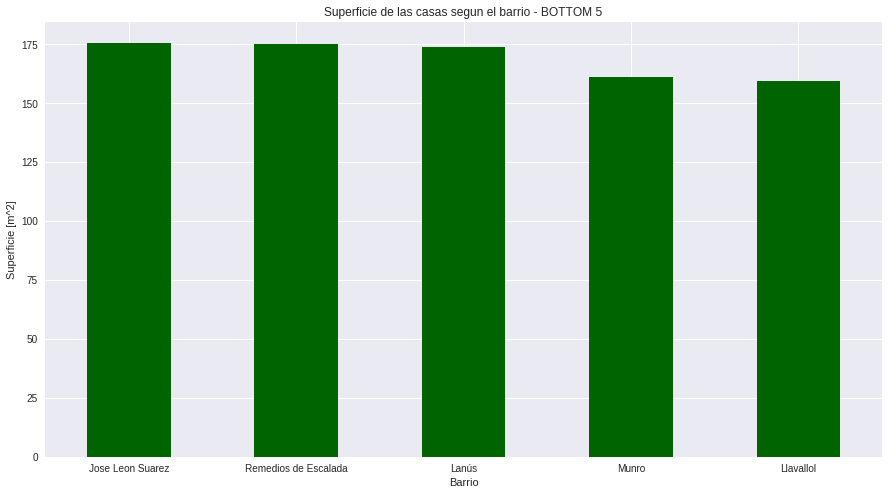
\includegraphics[width=\textwidth]{images/houseSurfaceBottomBar}
				  	\end{center}
				  	\begin{center}
   		    				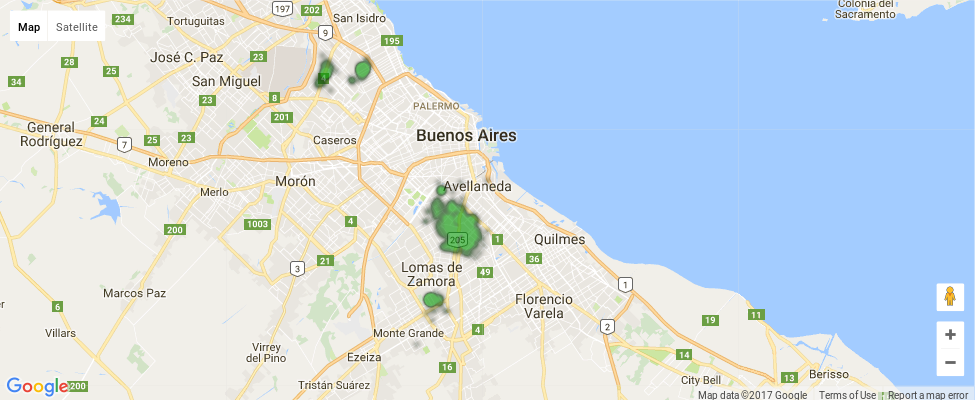
\includegraphics[width=\textwidth]{images/houseSurfaceBottomMap}
				  	\end{center}
				\subsubsection{PHs}
					\begin{center}
   		    				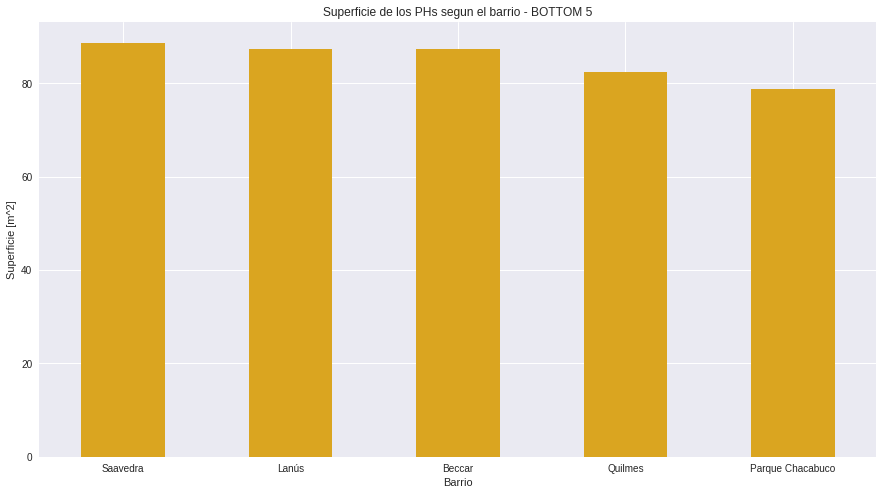
\includegraphics[width=\textwidth]{images/phSurfaceBottomBar}
				  	\end{center}
				  	\begin{center}
   		    				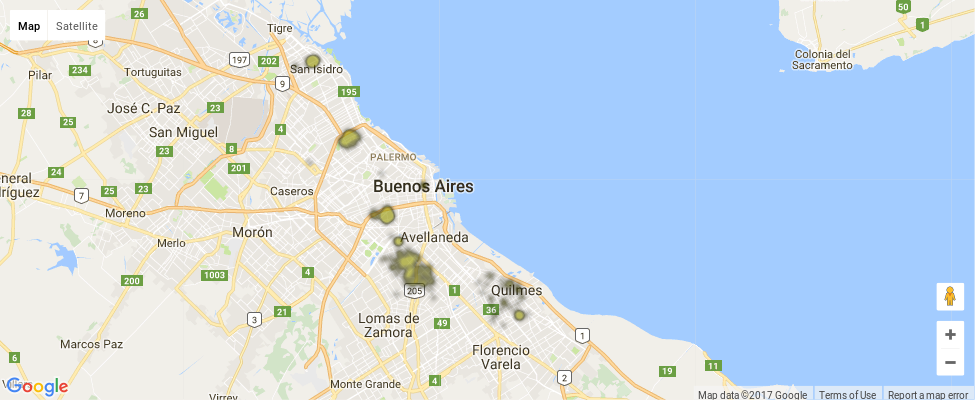
\includegraphics[width=\textwidth]{images/phSurfaceBottomMap}
				  	\end{center}
				\subsubsection{Departamentos}
					\begin{center}
   		    				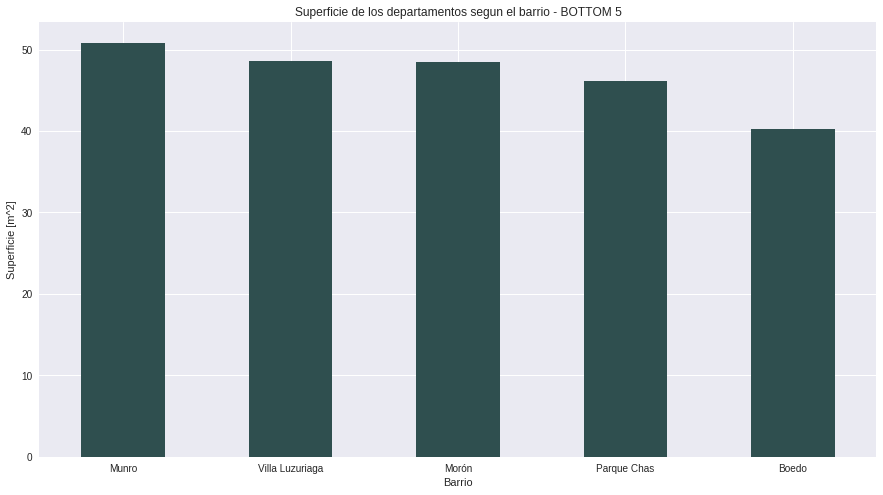
\includegraphics[width=\textwidth]{images/apartmentSurfaceBottomBar}
				  	\end{center}
				  	\begin{center}
   		    				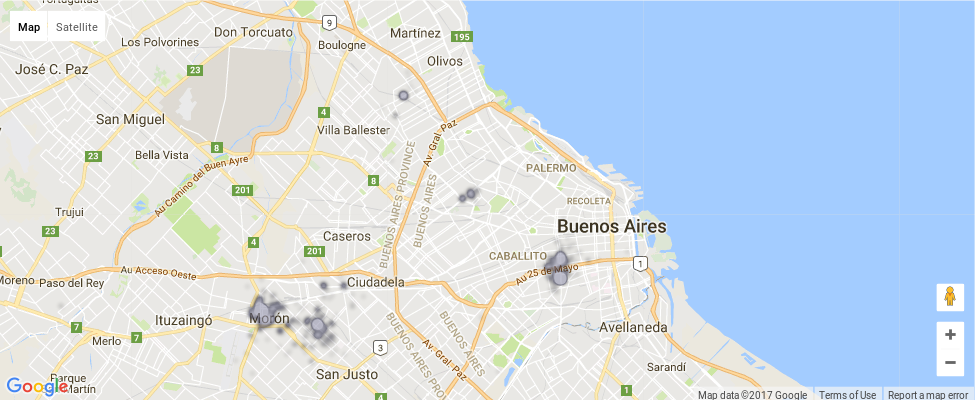
\includegraphics[width=\textwidth]{images/apartmentSurfaceBottomMap}
				  	\end{center}
				\subsubsection{Locales}
					\begin{center}
   		    				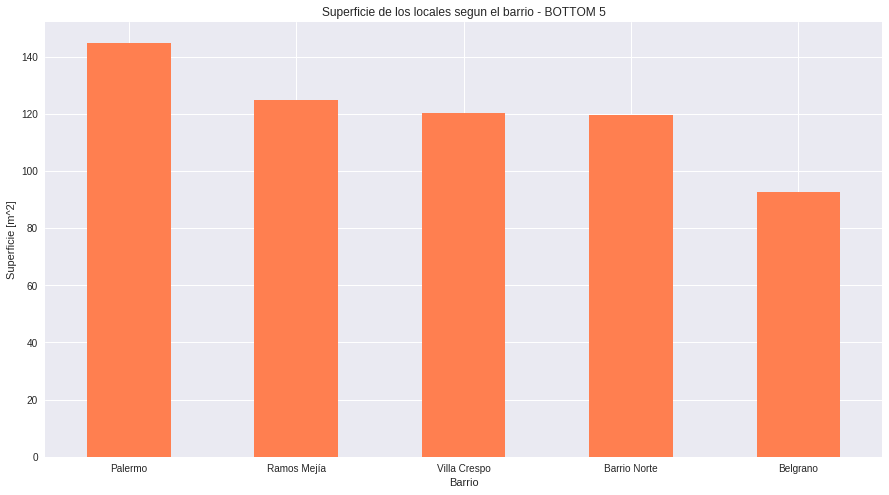
\includegraphics[width=\textwidth]{images/storeSurfaceBottomBar}
				  	\end{center}
				  	\begin{center}
   		    				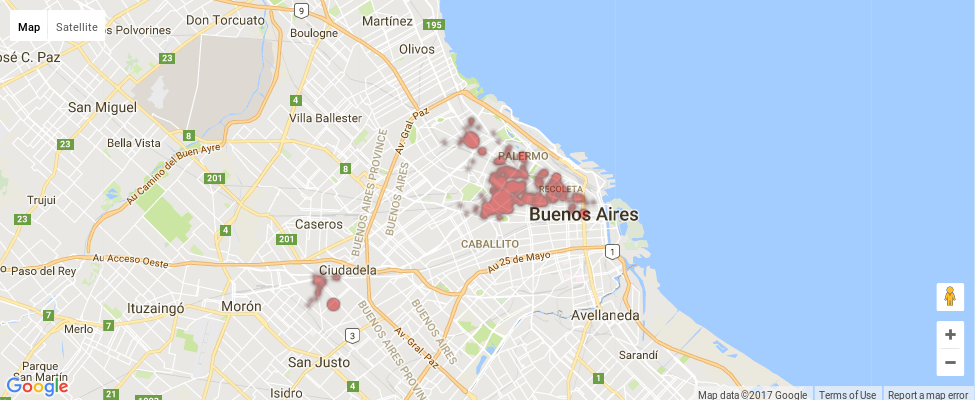
\includegraphics[width=\textwidth]{images/storeSurfaceBottomMap}
				  	\end{center}
		\section{Tipos de propiedades y sus precios}
			\subsection{¿Dónde están las propiedades más caras según su tipo?}
				El objetivo de esta sección es analizar donde se ubican las propiedades mas caras, dependiendo del tipo que sean. \\
				Vale destacar, que para realizar el análisis próximo a presentarse, primero se filtro por tipo de propiedad y luego se agrupo por barrio, dejando el promedio y la cantidad de entradas como valor. Para todos los casos a presentarse a continuación, se filtro con un mínimo de entradas igual a 20.
				 			
				\subsubsection{Casas}
				Para el caso particular de las casas, se realizo un \emph{TOP 5} obteniendo los siguientes resultados:
				
					\begin{center}
						\begin{tabular}{ |c|c| }
							\hline
							\multicolumn{2}{|c|}{TOP 5 de las casas mas caras}\\
							\hline
							\hline
							Barrio & Precio(USD)\\
							\hline
							 Belgrano & 2610.771984 \\
							 Palermo & 2598.033402 \\
							 Santa Barbara Barrio Cerrado & 2418.894358 \\
							 Nuñez & 2270.098719 \\
							 Barrio Los Castores & 2223.561320 \\
							\hline
						\end{tabular}
					\end{center}
				
				Se puede observar en la tabla, que la diferencia entre los primeros 2 barrios es muy pequeña, pero aumenta a mas de 1000 Usd con los ultimos 3 de la tabla.
				
				\begin{center}
   		    				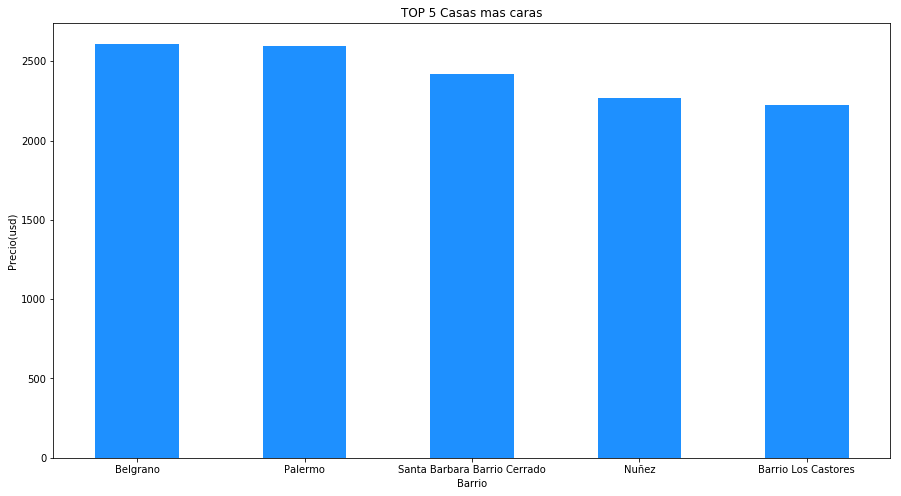
\includegraphics[width=\textwidth]{images/topCc}
				\end{center}
				
				Finalmente, se añade la ubicación de dichas casas:
				
				\begin{center}
   		    				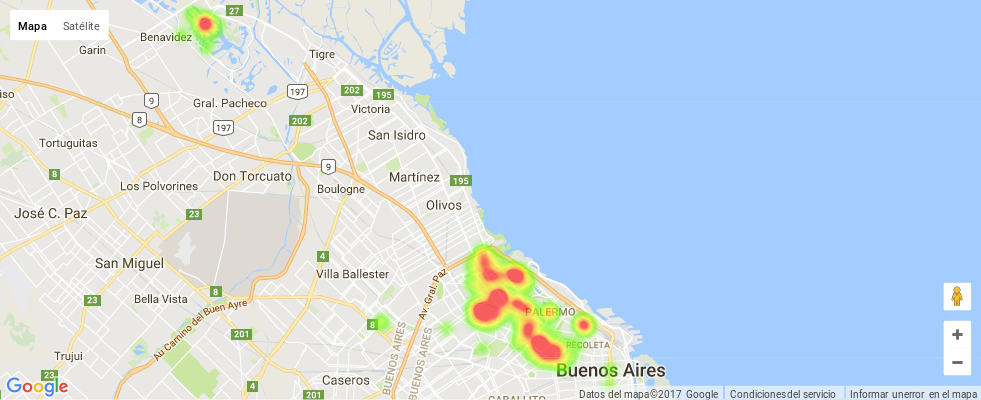
\includegraphics[width=\textwidth]{images/ubicCc}
				\end{center}
 
				Entonces se puede notar que las casas mas caras, como se analizo en el capitulo anterior, se encuentran en las zonas donde tanto el precio por metro cuadrado, como el precio aproximado de las viviendas es mas elevado, salvo por el Barrio Santa Barbara. Este último, es un barrio cerrado ubicado en Benavidez. 


				\subsubsection{PHs}
				Para los PHs el \emph{TOP 5}, entrego los siguientes resultados:
				
					\begin{center}
						\begin{tabular}{ |c|c| }
							\hline
							\multicolumn{2}{|c|}{TOP 5 de las PHs mas caros}\\
							\hline
							\hline
							Barrio & Precio(USD)\\
							\hline
							Palermo Soho & 2657.484915 \\
							Coghlan & 2485.627732 \\
							Belgrano & 2435.721287 \\
							Palermo & 2382.434241 \\
							Nuñez & 2275.340938 \\
							\hline
						\end{tabular}
					\end{center}
				
				\begin{center}
   		    				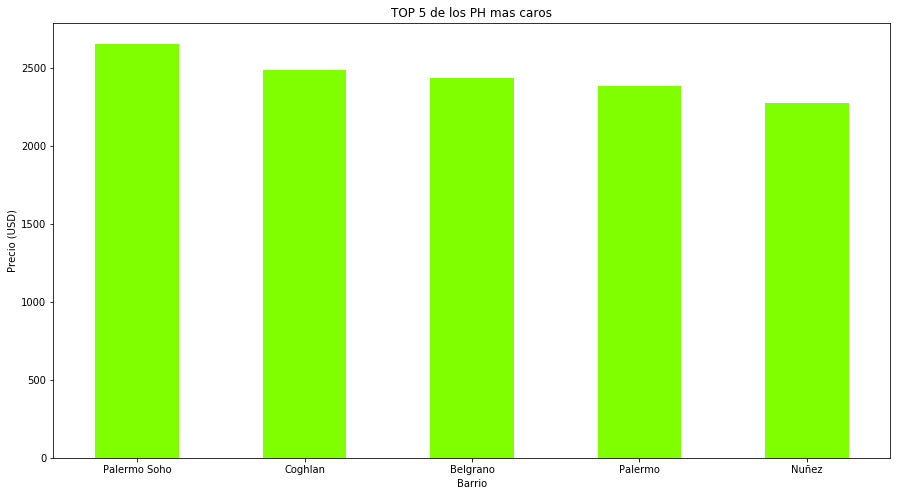
\includegraphics[width=\textwidth]{images/topPHc}
				\end{center}
				
				Tal como se puede ver en el gráfico y en la tabla, la mayor diferencia se presenta entre el primero y el segundo, siendo esta de 172 Usd.\\				
				Finalmente, se añade la ubicación de dichos PH:
				
				\begin{center}
   		    				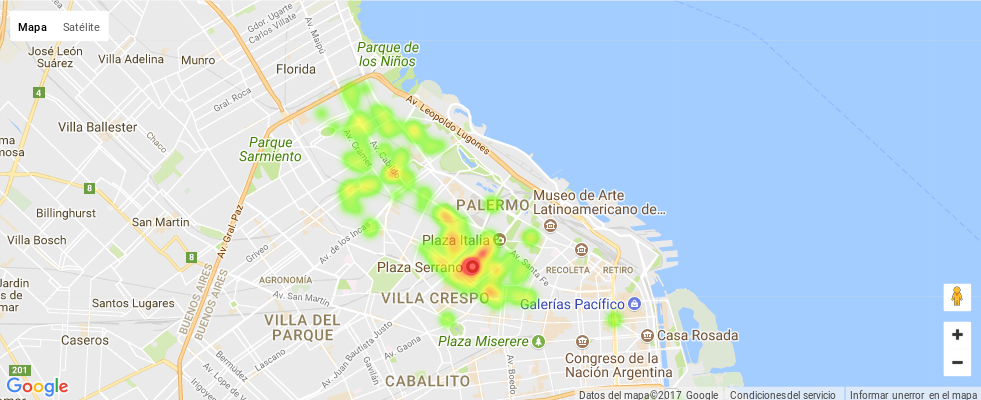
\includegraphics[width=\textwidth]{images/ubicPHc}
				\end{center}	
				
				Si bien los datos son consistentes respecto con el análisis hecho en el capitulo anterior, uno esperaría que la mayor cantidad de PHs se ubicara en GBA. Como podemos ver, esta hipótesis no es valida.
				
				\subsubsection{Departamentos}
				Para los Departamentos el \emph{TOP 5}, arrojo los siguientes resultados:
				
					\begin{center}
						\begin{tabular}{ |c|c| }
							\hline
							\multicolumn{2}{|c|}{TOP 5 de las Departamentos mas caros}\\
							\hline
							\hline
							Barrio & Precio(USD)\\
							\hline
							Puerto Madero & 5681.950867 \\
							Palermo Chico & 4372.664773 \\
							Las Cañitas & 3625.253679 \\
							Vicente López & 3365.357986 \\
							Olivos & 3307.502819 \\
							\hline
						\end{tabular}
					\end{center}
				
				\begin{center}
   		    				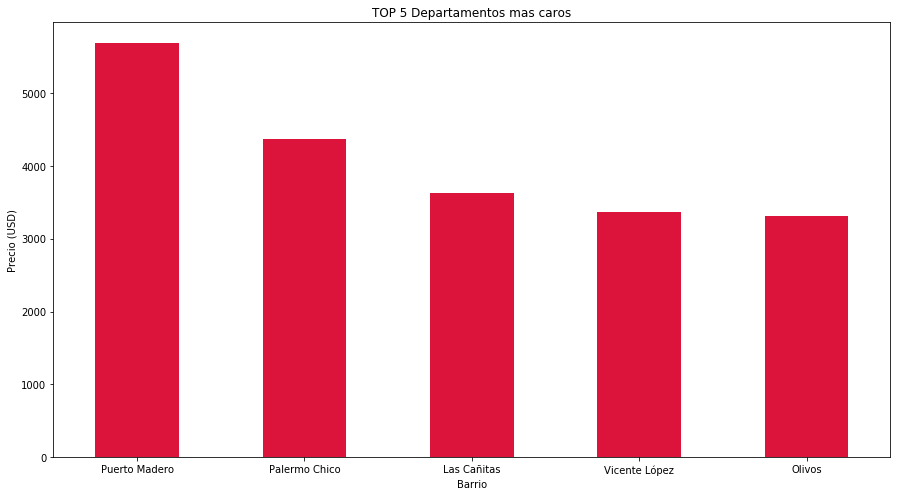
\includegraphics[width=\textwidth]{images/topDc}
				\end{center}
				
				Se puede observar claramente en el gráfico que, hay una diferencia muy abrupta entre las primeras 3 ubicaciones, estabilizándose hacia el final de la tabla.\\				
				Finalmente, se añade la ubicación de dichos Departamentos:
				
				\begin{center}
   		    				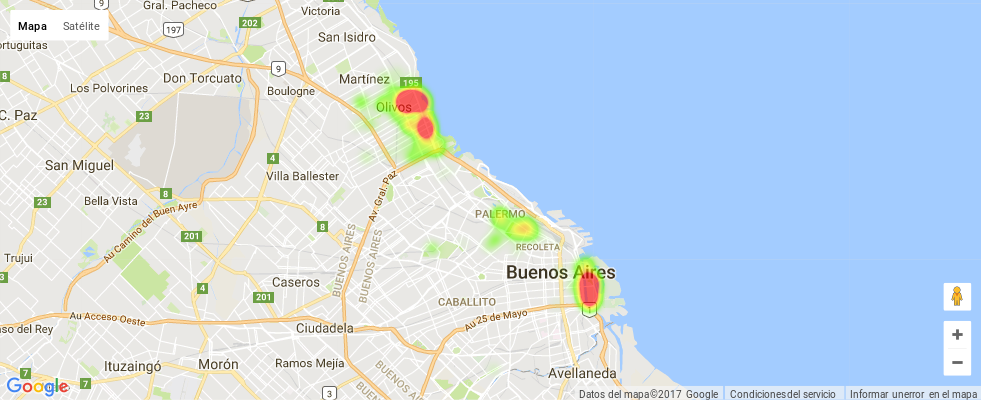
\includegraphics[width=\textwidth]{images/ubicDc}
				\end{center}	
				
				Como se puede observar en el gráfico anterior, se tiene la mayor cantidad departamentos con precio elevado en CABA. También hay que notar, que los departamentos que están en GBA se encuentran en barrios cercanos a CABA.
				
				\subsubsection{Locales}
				
					Para los Locales se obtuvieron los siguientes resultados del \emph{TOP 5}:
				
					\begin{center}
						\begin{tabular}{ |c|c| }
							\hline
							\multicolumn{2}{|c|}{TOP 5 de las Locales mas caros}\\
							\hline
							\hline
							Barrio & Precio(USD)\\
							\hline
							Palermo & 3944.669361 \\
							Recoleta & 3851.392729 \\
							Belgrano & 3361.595914 \\
							Villa Crespo & 3280.676456 \\
							Ramos Mejía & 3167.439625 \\
							\hline
						\end{tabular}
					\end{center}
				
				\begin{center}
   		    				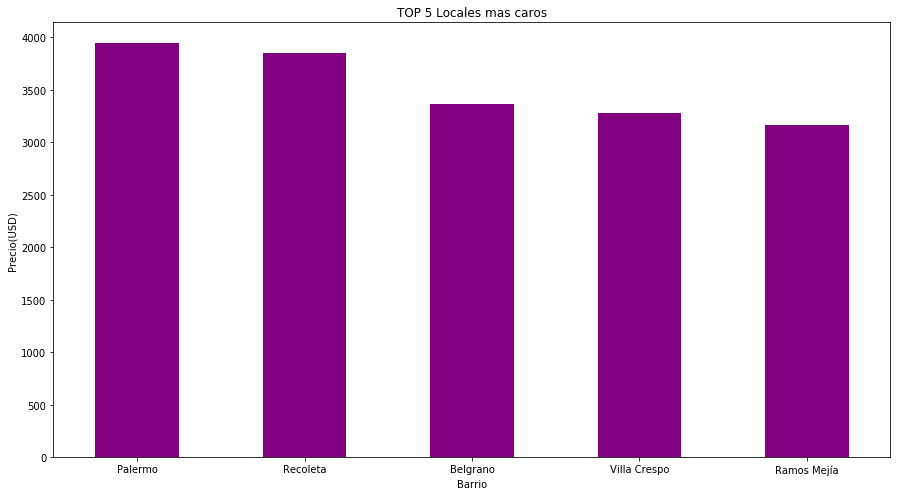
\includegraphics[width=\textwidth]{images/topLc}
				\end{center}
				
				Se puede ver en la tabla y el gráfico, que la mayor diferencia se presenta entre los primeros 2 y los últimos 3.\\				
				Finalmente, se añade la ubicación de los Locales mas caros:
				
				\begin{center}
   		    				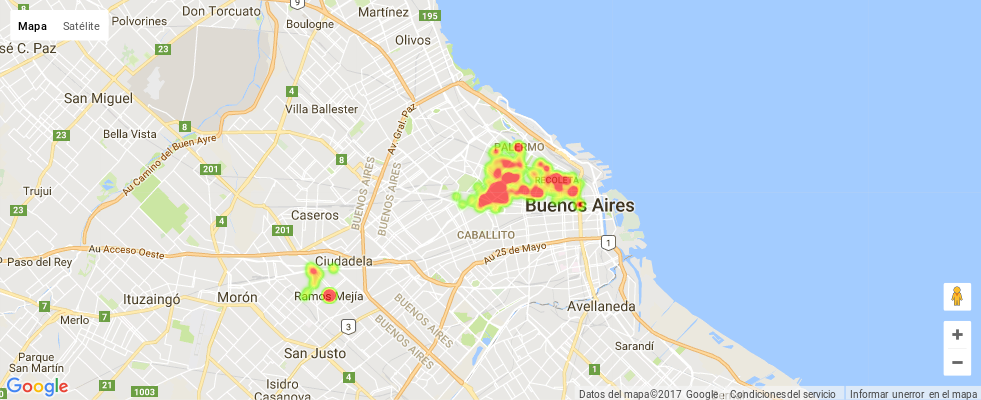
\includegraphics[width=\textwidth]{images/ubicLc}
				\end{center}	
				
				Como se puede observar en el gráfico anterior, los locales mas caros se concentran en CABA, salvo por los últimos 2 datos de la tabla.
				
				
			\subsection{¿Dónde están las propiedades más baratas según su tipo?}
				En esta sección se propone analizar donde se ubican las propiedades mas baratas. \\
				En dicha sección se realizaron los mismos filtrados que para las propiedades mas caras.
				 							
				\subsubsection{Casas}
				
				Se realizo un \emph{TOP 5} obteniendo los siguientes resultados para las casas:
				
					\begin{center}
						\begin{tabular}{ |c|c| }
							\hline
							\multicolumn{2}{|c|}{TOP 5 de las casas mas baratos}\\
							\hline
							\hline
							Barrio & Precio(USD)\\
							\hline
							Villa Udaondo & 864.062761 \\
							Valentín Alsina 	& 863.197187 \\
							Villa Madero & 862.186426 \\
							San Martín & 830.209696 \\
							La Tablada & 807.027363 \\
							\hline
						\end{tabular}
					\end{center}
				
				
				\begin{center}
   		    				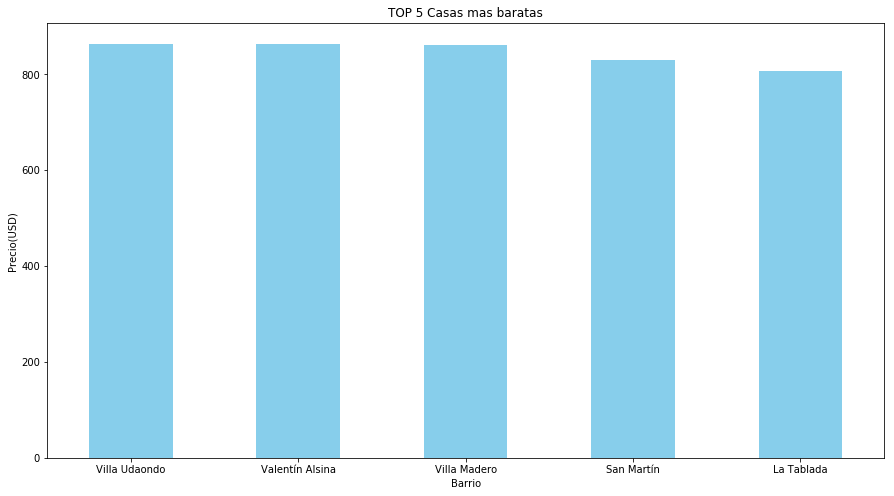
\includegraphics[width=\textwidth]{images/topCb}
				\end{center}
				
				Se puede observar, que la diferencia entre los distintos barrios es muy pequeña. Dicha diferencia, no supera los 60 Usd entre el primero y el último.
				Finalmente, se añade la ubicación de dichas casas:
				
				\begin{center}
   		    				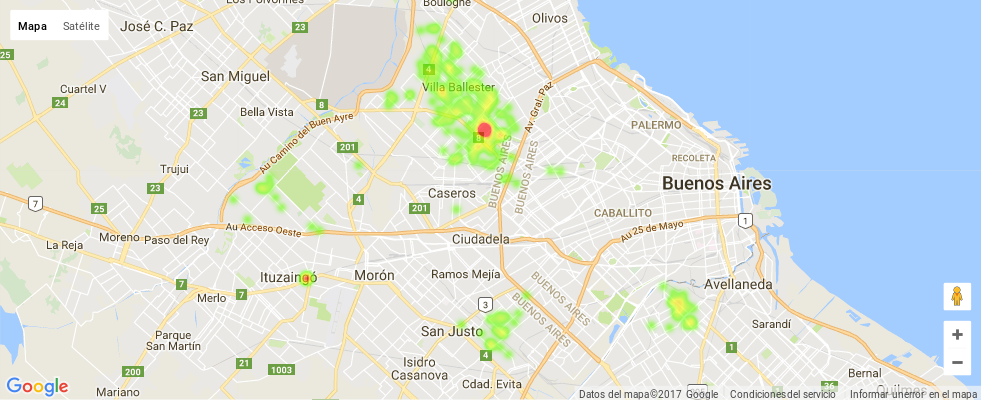
\includegraphics[width=\textwidth]{images/ubicCb}
				\end{center}
 
				Se puede notar, que las casas con menores precios se ubican en GBA, lo cual era esperable, ya que concuerda con el análisis de precio por metro cuadrado y de precio aproximado.
				
				\subsubsection{PHs}
				
					Para los PHs el se obtuvieron los siguientes resultados del \emph{TOP 5}:
				
					\begin{center}
						\begin{tabular}{ |c|c| }
							\hline
							\multicolumn{2}{|c|}{TOP 5 de las PHs mas baratos}\\
							\hline
							\hline
							Barrio & Precio(USD)\\
							\hline
							Villa Bosch & 1157.563280 \\
							Lanús Oeste & 1109.922068 \\
							El Palomar & 1103.662526 \\														
							Ituzaingó & 1021.952671 \\
							San Martín & 947.012756 \\

							\hline
						\end{tabular}
					\end{center}
				
				\begin{center}
   		    				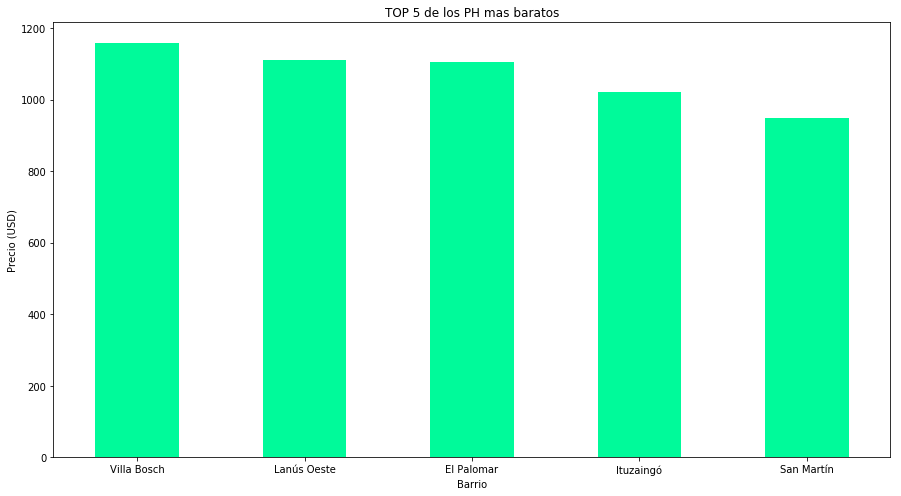
\includegraphics[width=\textwidth]{images/topPHb}
				\end{center}
				
				Se puede observar que se obtienen diferencias muy cercanas entre las distintas zonas, salvo entre la segunda y tercera donde la diferencia es mucho menor al resto de la tabla.
				
				\begin{center}
   		    				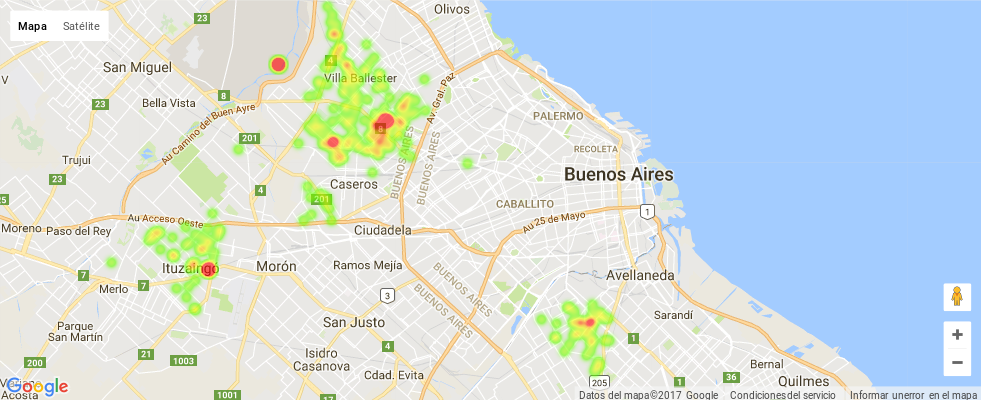
\includegraphics[width=\textwidth]{images/ubicPHb}
				\end{center}	
				
				Como se puede ver en este gráfico, los resultados son totalmente esperables, ya que los PHs con menor precio se encuentran ubicados en \code{CABA}
				
				\subsubsection{Departamentos}
				
					Para los Departamentos el \emph{TOP 5}, entrego los siguientes resultados:
				
					\begin{center}
						\begin{tabular}{ |c|c| }
							\hline
							\multicolumn{2}{|c|}{TOP 5 de las Departamentos mas baratos}\\
							\hline
							\hline
							Barrio & Precio(USD)\\
							\hline
							Pompeya & 1205.936453 \\
							Bs.As. G.B.A. Zona Oeste & 1173.854686 \\
							Hurlingham & 1144.014297 \\
							Pilar Village & 1131.876143 \\
							José C Paz & 1057.673806 \\
						\end{tabular}
					\end{center}
				
				
				\begin{center}
   		    				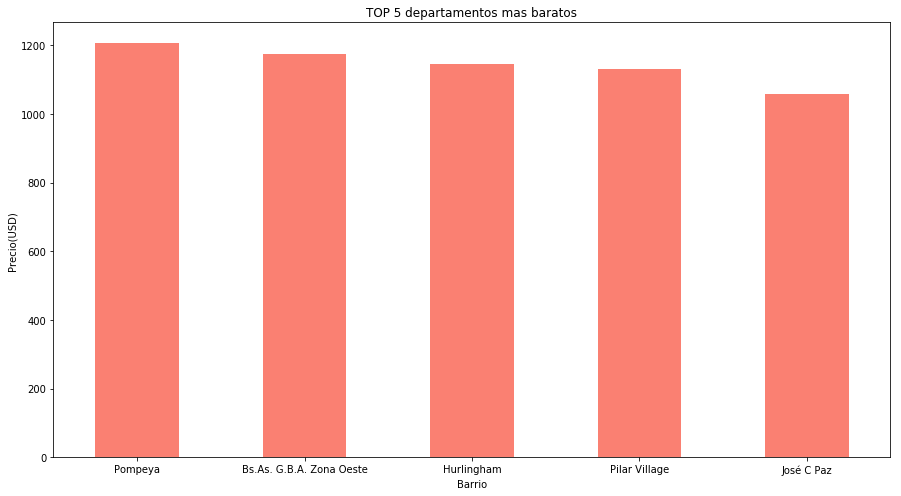
\includegraphics[width=\textwidth]{images/topDb}
				\end{center}
				
				Se puede apreciar que las diferencias entre los barrios de la tabla, son muy parecidas entre sí.\\		
				Finalmente, se añade la ubicación de dichos Departamentos:
				
				\begin{center}
   		    				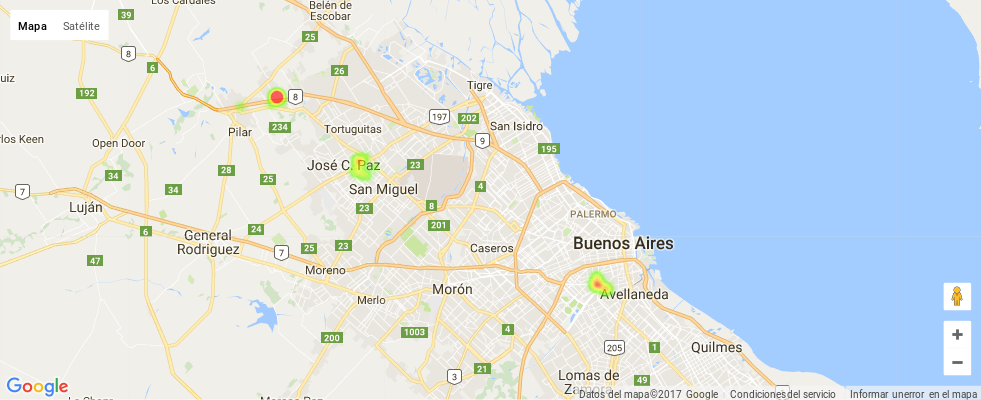
\includegraphics[width=\textwidth]{images/ubicDb}
				\end{center}	
				
				Se puede observar en el gráfico, que los departamentos con menores precios están ubicados únicamente en GBA. Lo cual es esperable, debido al análisis realizado en el capitulo anterior y lo obtenido con los departamentos mas caros.
				
				\subsubsection{Locales}
				
					Para los Locales el \emph{TOP 5} lanzo los siguientes resultados:
				
					\begin{center}
						\begin{tabular}{ |c|c| }
							\hline
							\multicolumn{2}{|c|}{TOP 5 de las Locales mas baratos}\\
							\hline
							\hline
							Barrio & Precio(USD)\\
							\hline
							San Justo & 1575.904794 \\
							Mataderos & 1544.208404 \\
							Temperley & 1509.434793 \\
							General San Martín & 1478.113426 \\
							Villa Ballester 	& 1264.444924 \\
							\hline
						\end{tabular}
					\end{center}
				
				\begin{center}
   		    				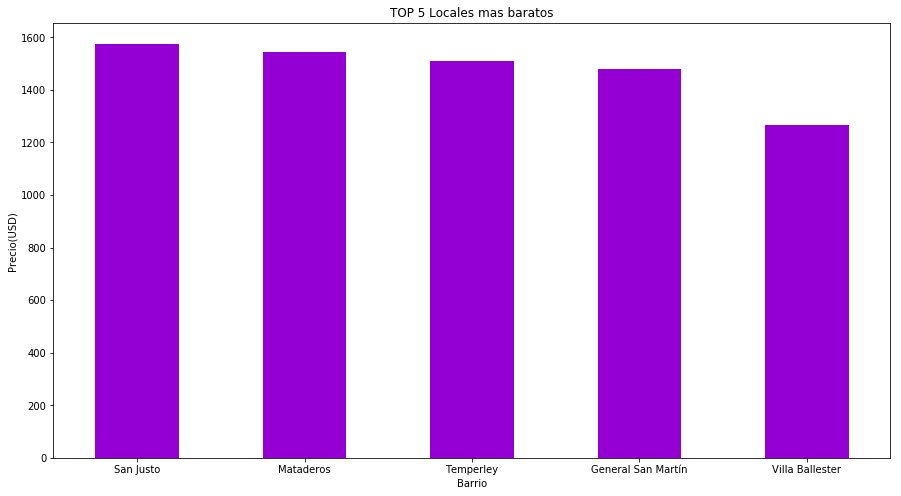
\includegraphics[width=\textwidth]{images/topLb}
				\end{center}
				
				Se puede ver que la mayor diferencia de precios entre las distintas localidades, se da entre las últimas 2 de la tabla, siendo las diferencias del resto muy similares.\\				
				Finalmente, se añade la ubicación de los Locales mas baratos:
				
				\begin{center}
   		    				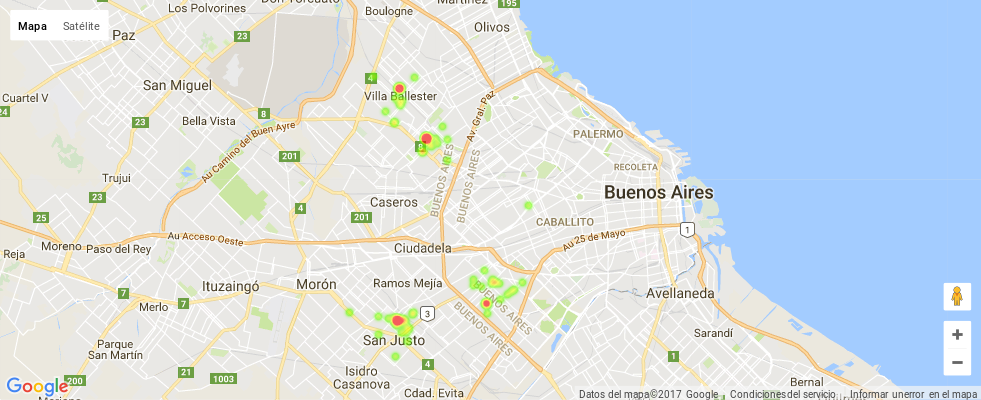
\includegraphics[width=\textwidth]{images/ubicLb}
				\end{center}	
				
				Como era de esperar, los Locales mas baratos se encuentran ubicados en la zona de CABA.
				
		
		\section{Tipos de propiedades y sus ubicaciones}
			\subsection{¿En qué lugar hay más propiedades de cada tipo?}
				%Top 5 (heat-map)
				\subsubsection{Casas}
				\subsubsection{PHs}
				\subsubsection{Departamentos}
				\subsubsection{Locales}
		
		
		\section{Variación del precio total a través de los años}
			\subsection{Casas}
			\subsection{PHs}
			\subsection{Departamentos}
			\subsection{Locales}
		
		
		\section{Variación del precio por $m^2$ a través de los años}
			En esta sección, el objetivo es analizar la variación del precio por $m^2$ de cada uno de los tipos de propiedad
			disponibles. Se espera que, en todos los casos, la variación sea creciente alcanzando su máximo en 2017. De todas formas,
			el objetivo es ver cuál varió más y cómo fue dicha variación.
			\subsection{¿Cuál fue el tipo de propiedad más caro en cada año?}
				En este caso, la pregunta es: año a año, cuál fue el tipo de propiedad con mayor precio por $m^2$.
				\subsubsection{2013}
					Para el año 2013, podemos ver que los departamentos fueron los más caros, teniendo en segundo lugar a los
					PHs, en tercero a las casas y finalmente a los locales.
					\begin{center}
   		    				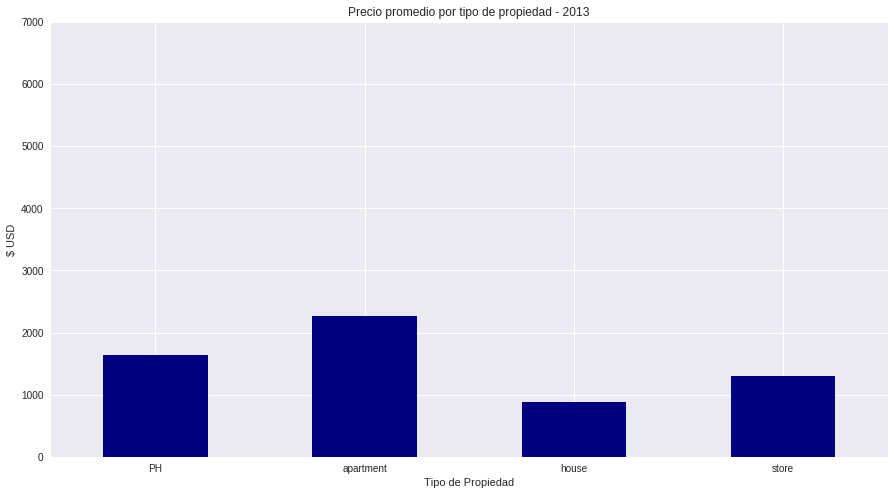
\includegraphics[width=\textwidth]{images/propPrice2013}
				  	\end{center}
				\subsubsection{2014}
					En 2014 se observa un aumento en los precios de los locales mientras que el resto de los tipos de propiedad
					se mantienen casi igual.
					\begin{center}
   		    				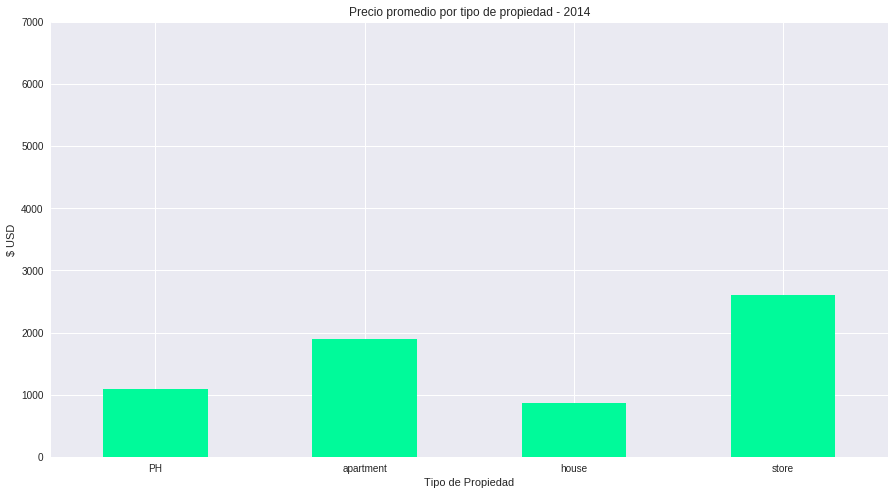
\includegraphics[width=\textwidth]{images/propPrice2014}
				  	\end{center}
				\subsubsection{2015}
					Ahora, en el año 2015, podemos ver que la forma es igual que en 2014 aunque con precios levemente más elevados.
					\begin{center}
   		    				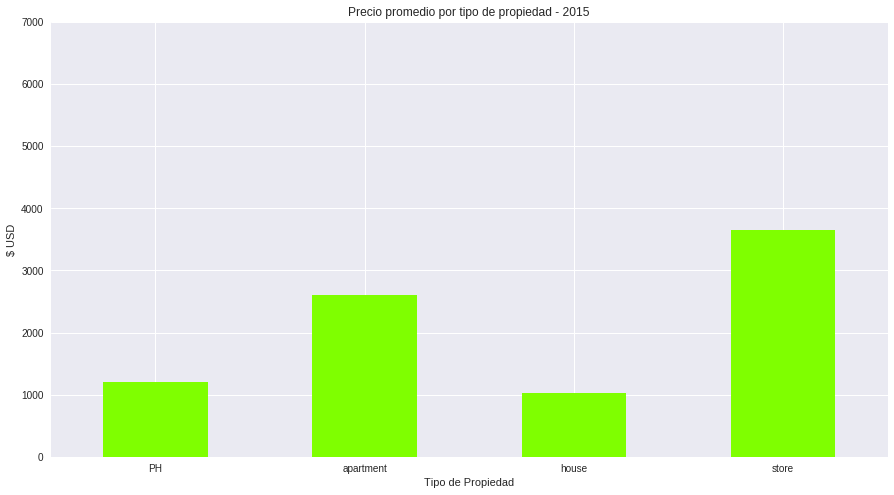
\includegraphics[width=\textwidth]{images/propPrice2015}
				  	\end{center}
				\subsubsection{2016}
					Para 2016 se encuentra una suba en los precios en general y un ascenso al segundo puesto de los PHs, mientras
					que los locales siguen en el primer puesto.
					\begin{center}
   		    				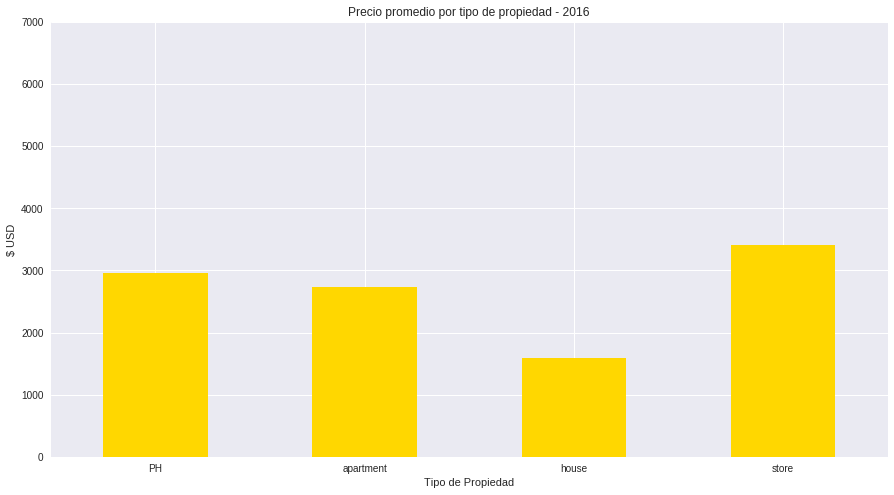
\includegraphics[width=\textwidth]{images/propPrice2016}
				  	\end{center}
				\subsubsection{2017}
					Finalmente, en 2017 vuelven a tomar el segundo puesto los departamentos y se ve el aumento más grande en los
					cuatro años, llegando los locales a un promedio de $7000$USD.
					\begin{center}
   		    				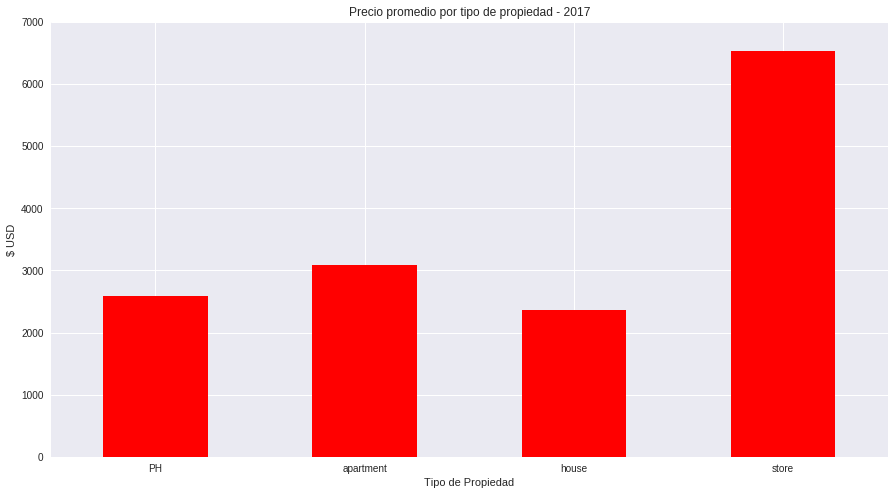
\includegraphics[width=\textwidth]{images/propPrice2017}
				  	\end{center}
			\subsection{Casas}
				En el caso de las casas nos encontramos con una variación muy pequeña para el intervalo $[2013, 2015]$ y mucho
				más marcada para los últimos dos años. De todos modos, en total, la variación es de aproximadamente $1500$USD.
				\begin{center}
   		    			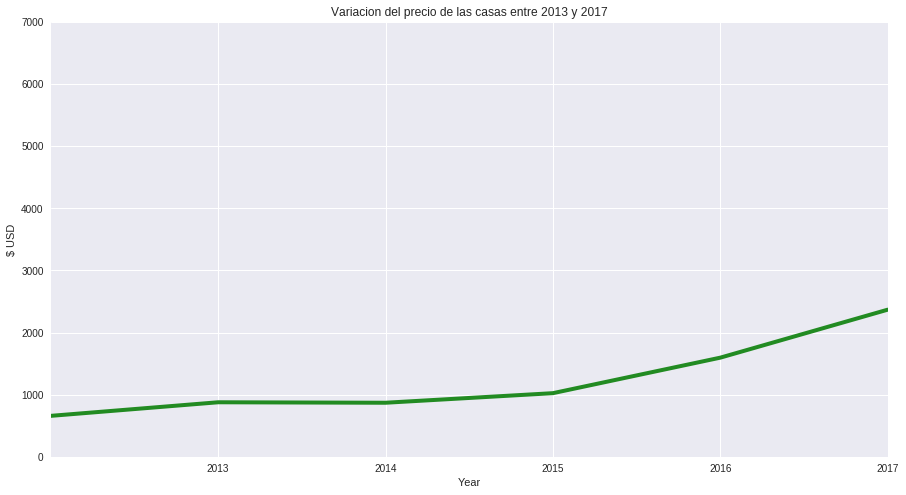
\includegraphics[width=\textwidth]{images/houseVariation}
				\end{center}
			\subsection{PHs}
				En este caso, si bien la variación es de aproximadamente $1000$USD, vemos que en el año 2015 hubo un aumento del
				valor de los PHs de aproximadamente $2000$USD, con un posterior decrecimiento durante 2016 y 2017. Este tipo
				de propiedad tuvo descensos y ascensos alternados, uno cada año.
				\begin{center}
   		    			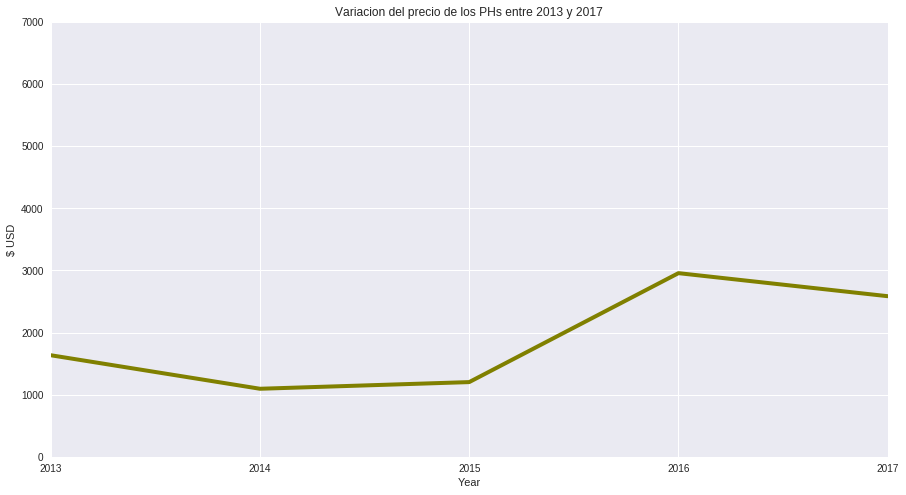
\includegraphics[width=\textwidth]{images/phVariation}
				\end{center}
			\subsection{Departamentos}
				Nuevamente encontramos un aumento de aproximadamente $1000$USD en el valor de los departamentos entre los cuatro
				años, con un descenso entre 2013 y 2014 pero con un aumento en los años siguientes.
				\begin{center}
   		    			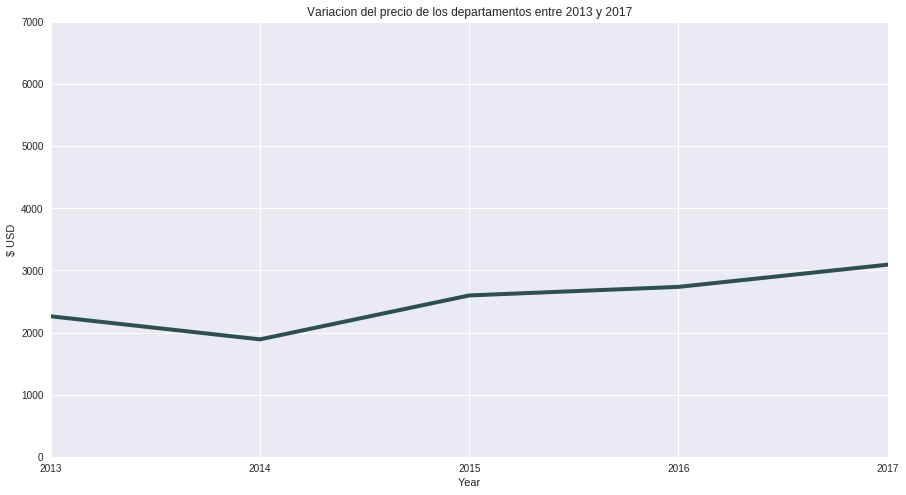
\includegraphics[width=\textwidth]{images/apartmentsVariation}
				\end{center}
			\subsection{Locales}
				Finalmente, en el caso de los locales, podemos ver que el aumento es exageradamente grande (aproximadamente del
				$600\%$) en el paso de los últimos cuatro años. Se puede observar un aumento con una gran pendiente en los primeros
				dos años, un leve descenso entre 2015 y 2016 y finalmente un nuevo aumento importante. \\
				\tab Consideramos que la magnitud de esta variación se puede deber a dos cosas; la primera es que efectivamente los
				precios por $m^2$ de los locales haya aumentado de esta manera y la segunda es que los numeros obtenidos se deban
				a la poca cantidad de entradas que se poseen de los primeros tres años. De todas maneras, reforzando la primer 
				opción, el año 2016 y 2017 poseen una cantidad de entradas muy similar y el cambio es de unos $3000$USD.
				\begin{center}
   		    			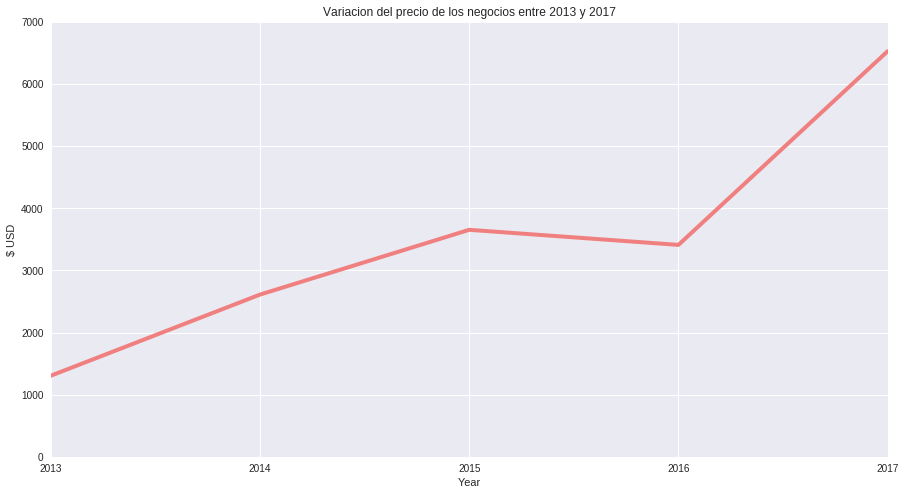
\includegraphics[width=\textwidth]{images/storeVariation}
				\end{center}
			\subsection{Análisis conjunto}
				Por último, uniremos los previos cuatro gráficos para un análisis conjunto de los datos obtenidos.
				\begin{center}
   		    			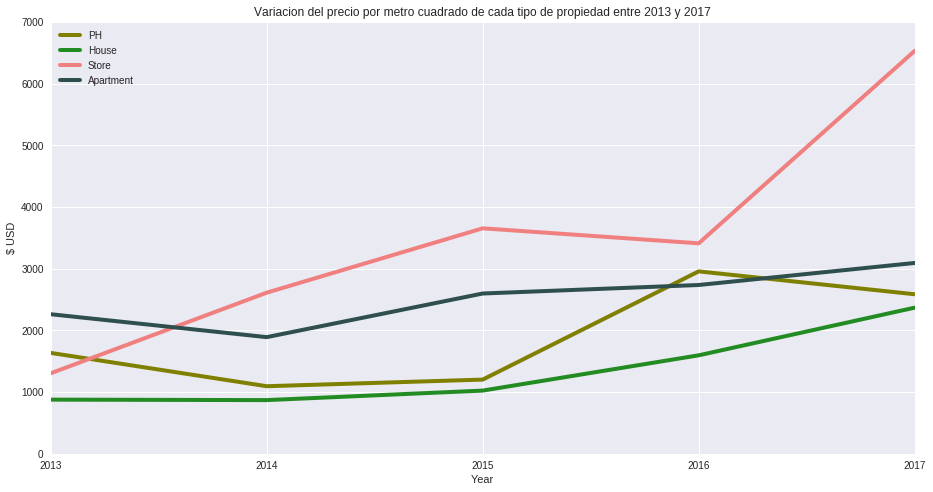
\includegraphics[width=\textwidth]{images/jointVariation}
				\end{center}
				\tab Aquí se puede ver que todas las viviendas tienen una variación similar y que su precio en 2017 es muy similar.
				Por otro lado, los locales destacan por su bajo comienzo (casi último) y su alto final (primero con más de $3000$USD
				de diferencia). \\
				\tab Podemos concluír, entonces, notando que la relación de precios se mantuvo con el pasar de los años, manteniendo
				el orden de los precios. Es decir, los departamentos son los más caros, seguidos por los PHs y terminando con 
				las casas pero con precios cada vez mayores, como se esperaba.
		
\end{document}